\chapter{Solution}
\label{solution}

The previous chapters have shown how the single-phase flow equation has been defined, discretized, simplified, linearized, and linked with the well model. Then it is possible to initialize the simulation and advance it in time. This chapter is composed of two sections, the equilibration process and the advancement in time. The first shows how the pressure distribution in the reservoir will be calculated for time zero. The second shows how the pressure at the next time step will be calculated, thus advancing the simulation in time. Finally, the last section shows how the simulator has been validated, by comparing its results with reliable data.

\section{Equilibration Process}

At the beginning of the simulation, the initial pressures at each grid block $p_{i,j,k}^{n=0}$ are usually unknown. Thus, it is necessary to calculate them before advancing in time. Normally, the user of a reservoir simulator has to input one or more value of pressures $P^0$ at reference depths $Z^0$, in what is called an equilibration table. Then the simulator can compute the initial pressure distribution in the entire reservoir by applying hydrostatics. This is known as the equilibration process and will be described in this section. Assuming a hydrostatic equilibrium at the time zero, $\nabla \Phi = 0$, Eq. \ref{eq:10} can be rewritten as:
\begin{align}
\label{00}
\nabla \Phi=\nabla p - \gamma \nabla Z = 0.
\end{align}
Thus:
\begin{align}
\label{00aaa}
P^0 - p_{i,j,k} - \gamma_{i,j,k}(Z^0 - Z_{i,j,k}) = 0,
\end{align}
which can be rewritten as:
\begin{align}
\label{00aa}
p_{i,j,k}=P^0+\gamma_{i,j,k}(Z_{i,j,k}-Z^0),
\end{align}
Since the scenario considers a compressible fluid, its specific weight $\gamma$ can change with pressure. Thus, it would be necessary to calculate both the pressure and the specific weight.  Since they are mutually dependent unknowns, it is necessary to perform an iteration. Utilizing an index $\nu$ for the iteration level, the specific weight $\gamma$ will be evaluated in level $\nu$ and the pressure $p_{i,j,k}$ will be evaluated in the level $\nu+1$:
\begin{align}
\label{00a}
p^{(\nu+1)}_{i,j,k}=P^0+\gamma^{(\nu)}_{i,j,k}(Z_{i,j,k}-Z^0).
\end{align}
Figure \ref{cha:solution-fig:equilibration_process_iteration} shows this iterative process for a grid block $i$, $j$, $k$. $\epsilon$ is the tolerance of the iteration. It is set to be equal to $10^-8$ for all the simulations in this project. The equilibration process consists in applying this process for every grid block in the model. After that, the pressure initialization is done and it is then possible to advance the simulation in time.

\nomenclature[G]{$\epsilon$}{Tolerance of the iteration}
\begin{figure}[H]
	\centering
	\begin{tikzpicture}[node distance=2cm]

\node (start) [startstop] {Begining of the iterative process};
\node (in1) [io, below of=start, yshift=-0.5cm] {$p_{i,j,k}^{\stackrel{\Large{\nu=0}}{n=0}} = 0$, $\gamma_{i,j,k}^{\stackrel{\Large{\nu=0}}{n=0}} = f(0)$, $\nu=0$, $P^0$, $Z^0$, $Z_{i,j,k}$};
\node (pro1) [process, below of=in1, yshift=-0.5cm] {$\gamma_{i,j,k}^{\stackrel{\Large{\nu}}{n=0}} = f(p_{i,j,k}^{\stackrel{\Large{\nu}}{n=0}})$};
\node (pro2) [process, below of=pro1] {$p_{i,j,k}^{\stackrel{\Large{\nu+1}}{n=0}} = P^0 + \gamma_{i,j,k}^{\stackrel{\Large{\nu}}{n=0}} (Z_{i,j,k} - Z^0)$};
\node (dec1) [decision, below of=pro2, yshift=-2cm] {$ \mid p_{i,j,k}^{\stackrel{\Large{\nu+1}}{n=0}} - p_{i,j,k}^{\stackrel{\Large{\nu}}{n=0}} \mid < \epsilon $ ?};
\node (pro2b) [process, right of=dec1, xshift=4cm] {$p_{i,j,k}^{\stackrel{\Large{\nu}}{n=0}} = p_{i,j,k}^{\stackrel{\Large{\nu+1}}{n=0}}$};
\node (pro3) [process, above of=pro2b, yshift=0cm] {$\nu = \nu + 1$};
\node (output) [io, below of=dec1, yshift=-2cm] {$p_{i,j,k}^{n=0} = p_{i,j,k}^{\stackrel{\Large{\nu+1}}{n=0}}$};
\node (stop2) [startstop, below of=output, yshift=0cm] {End of the iterative process};

\draw [arrow] (start) -- (in1);
\draw [arrow] (in1) -- (pro1);
\draw [arrow] (pro1) -- (pro2);
\draw [arrow] (pro2) -- (dec1);
\draw [arrow] (dec1) -- node[anchor=east] {yes} (output);
\draw [arrow] (dec1) -- node[anchor=south] {no} (pro2b);
\draw [arrow] (pro2b) -- (pro3);
\draw [arrow] (pro3) |- (pro1);
\draw [arrow] (output) -- (stop2);

\end{tikzpicture}
	\caption{Iteration in the equilibration process.}
	\label{cha:solution-fig:equilibration_process_iteration}
\end{figure}


\section{Advancing in Time}

The \autoref{chapter:NF} presents the discretized and linearized form of the single-phase flow equation, Eq. \ref{matrix2}. After applying this equation to every grid block in the model, a linear system of equations is obtained. The \autoref{appendices_vis} shows how such a system is generated for a simple example of a tridimensional grid. This section shows how to utilize this linear system of equations to calculate the pressure at a new time step, hence, advancing the simulation in time.

Developing a linear algebra solver is not the focus of this project, thus, an external, open-source library has been utilized for solving the linear system of equations. This library is the UMFPACK, which stands for Unsymmetric, Multifrontal Sparse LU Factorization Package. It is a package that allows the solution of sparse linear systems by the method of LU factorization. \autoref{appendices_smr} shows how the linear system of equations has been represented in a compressed format (CSC) for enabling its solution with UMFPACK.

After the equilibration process has been finished, as described in the previous section, the initial pressure distribution in the reservoir $p_{i,j,k}^{n = 0}$ is obtained and then it is possible to calculate $p_{i,j,k}^{n + 1}$. Figure \ref{cha:solution-fig:advance_time_iteration} shows the algorithm for advancing the simulation in time, based on the Eq. \ref{matrix2}. The convergence of the process requires that the absolute value of the difference between the norms of the pressures at the iteration levels of $\nu+1$ and $\nu$ should be below the tolerance $\epsilon$, defined as $1 \times 10^{-8}$ for the models run in this project.
\nomenclature[S]{$\nu$}{Iteration index}
\nomenclature[S]{n}{Time index}
\begin{figure}[H]
	\centering
	\scalebox{.9}{\begin{tikzpicture}[node distance=2cm]

\node (start) [startstop] {Begining of the iterative process};
\node (in1) [io, below of=start, yshift=-0cm] {$p_{i,j,k}^{n}$, $\nu=0$};
\node (pro0) [process, below of=in1, yshift=-0cm] {$p^{\stackrel{(\nu)}{n+1}}_{i,j,k}$ = $p_{i,j,k}^{n=0}$};
\node (pro1) [process, below of=pro0, yshift=-1cm] {Calculate $A^{\stackrel{(\nu)}{n+1}}_{i,j,k}$, $B^{\stackrel{(\nu)}{n+1}}_{i,j,k}$, $N^{\stackrel{(\nu)}{n+1}}_{i,j,k}$, $S^{\stackrel{(\nu)}{n+1}}_{i,j,k}$, $E^{\stackrel{(\nu)}{n+1}}_{i,j,k}$, $W^{\stackrel{(\nu)}{n+1}}_{i,j,k}$, $C^{\stackrel{(\nu)}{n+1}}_{i,j,k}$ and $Q^{\stackrel{(\nu)}{n+1}}_{i,j,k}$ for $p^{\stackrel{(\nu)}{n+1}}_{i,j,k}$};
\node (pro2) [process, below of=pro1, yshift=-1cm] {solve $A x = B$, $p_{i,j,k}^{\stackrel{\Large{\nu+1}}{n+1}} = x$};
\node (dec1) [decision, below of=pro2, yshift=-2.5cm] {$\left| \| p_{i,j,k}^{\stackrel{\Large{\nu+1}}{n+1}} \| - \| p_{i,j,k}^{\stackrel{\Large{\nu}}{n+1}} \| \right| < \epsilon $ ?};
\node (pro2b) [process, right of=dec1, xshift=4.5cm] {$p_{i,j,k}^{\stackrel{\Large{\nu}}{n+1}} = p_{i,j,k}^{\stackrel{\Large{\nu+1}}{n+1}}$};
\node (pro3) [process, above of=pro2b, yshift=0cm] {$\nu = \nu + 1$};
\node (output) [io, below of=dec1, yshift=-2.5cm] {$p_{i,j,k}^{n+1} = p_{i,j,k}^{\stackrel{\Large{\nu+1}}{n+1}}$};
\node (stop2) [startstop, below of=output, yshift=0cm] {End of the iterative process};

\draw [arrow] (start) -- (in1);
\draw [arrow] (in1) -- (pro0);
\draw [arrow] (pro0) -- (pro1);
\draw [arrow] (pro1) -- (pro2);
\draw [arrow] (pro2) -- (dec1);
\draw [arrow] (dec1) -- node[anchor=east] {yes} (output);
\draw [arrow] (dec1) -- node[anchor=south] {no} (pro2b);
\draw [arrow] (pro2b) -- (pro3);
\draw [arrow] (pro3) |- (pro1);
\draw [arrow] (output) -- (stop2);

\end{tikzpicture}}
	\caption{Iteration for calculating the pressure distribution after a time step.}
	\label{cha:solution-fig:advance_time_iteration}
\end{figure}

\section{Validation}
A model should provide an accurate representation of a real system. Thus, an essential part of developing a reservoir simulation model is to ensure its accuracy, by validating its simulation results by comparing them with reliable data. In this project, this validation has been done by comparing the CSPF (a possible name for this simulator, which stands for Compressible, Single-Phase Flow simulator) simulation results with the ones generated by a industry-standard simulator for the same models. 

Two models have been utilized for this validation. The first is a buildup / drawdown well test scenario with homogeneous porosity and permeabilities. The second is a similar scenario, but with the only difference that the porosities and permeabilities are heterogeneous, generated by utilizing normal and log-normal distributions, respectively. Table \ref{tbl:2} shows the parameters utilized in the first validation model:
\nomenclature[A]{CSPF}{Compressible, Single-Phase Flow simulator}

\begin{table}[htbp]
	\centering
	\caption{Parameters of the homogeneous scenario for the validation.}
	\label{tbl:2}
	\begin{tabular}{c c}
		\toprule
		Parameter & Value (if applicable)\\
		\midrule
		Number of grid blocks in the $x$ direction & 15\\
		Number of grid blocks in the $y$ direction & 15\\
		Number of grid blocks in the $z$ direction & 10\\
		Boundary conditions & Sealed reservoir \\
		Well & Vertical well in the\\
		& center of the reservoir\\
		Completions & From the top to the\\
		& bottom of the reservoir\\
		Length of the grid blocks in the $x$ direction & 164.042 ft\\
		Length of the grid blocks in the $y$ direction & 164.042 ft\\
		Length of the grid blocks in the $z$ direction & 16.4042 ft\\
		Average porosity & 10\%\\
		Average horizontal permeability & 200 mD\\
		Average vertical permeability & 20 mD\\
		Formation compressibility & $1.31 x 10^{-4}$ psi$^{-1}$\\
		Fluid compressibility &  1.41 x 10$^{-5}$ psi$^{-1}$\\
		Depth of the topmost layer & 10,498.69 ft\\
		Reference depth for the initial pressure & 10,498.69 ft\\
		Initial pressure at the reference depth & 3,916.01 psi\\
		Well radius & 6 in\\
		Skin factor & -0.5\\
		\bottomrule
	\end{tabular}
\end{table}

The fluid utilized in both models has its proprieties described in Figure \ref{fig:30}. In the single-phase flow equation, the FVF, viscosity, and specific weight are obtained by applying a linear interpolation in these data. The fluid bubble point pressure is 3296.27 psi. This specific fluid model has been chosen since the pressure in the reservoir never reaches a value lower than its bubble point pressure and, therefore, would avoid a scenario of multiphase flow inferred by dissociated gas. The simulator developed in this project can not represent a condition of multiphase flow and would give unrealistic results.

\begin{figure}[h]
	\centering
	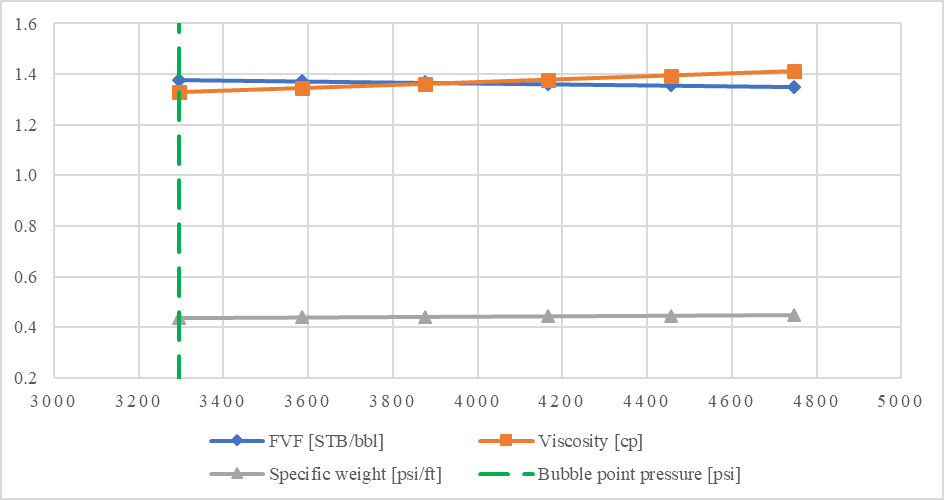
\includegraphics[width=1\linewidth]{Images/30}
	\caption{Fluid proprieties for the simulation.}
	\label{fig:30}
\end{figure}

The well has been initially set to be closed. At the time of 0.1 day, the well began producing at the flow rate of 2515.92 bbl/d, and ceased its production at the time 1.1 days. Thus, a drawdown/buildup test has been simulated. Figure \ref{fig:24} shows the bottom hole pressure for this test, both for the results from CSPF and IMEX.

\begin{figure}[h]
	\centering
	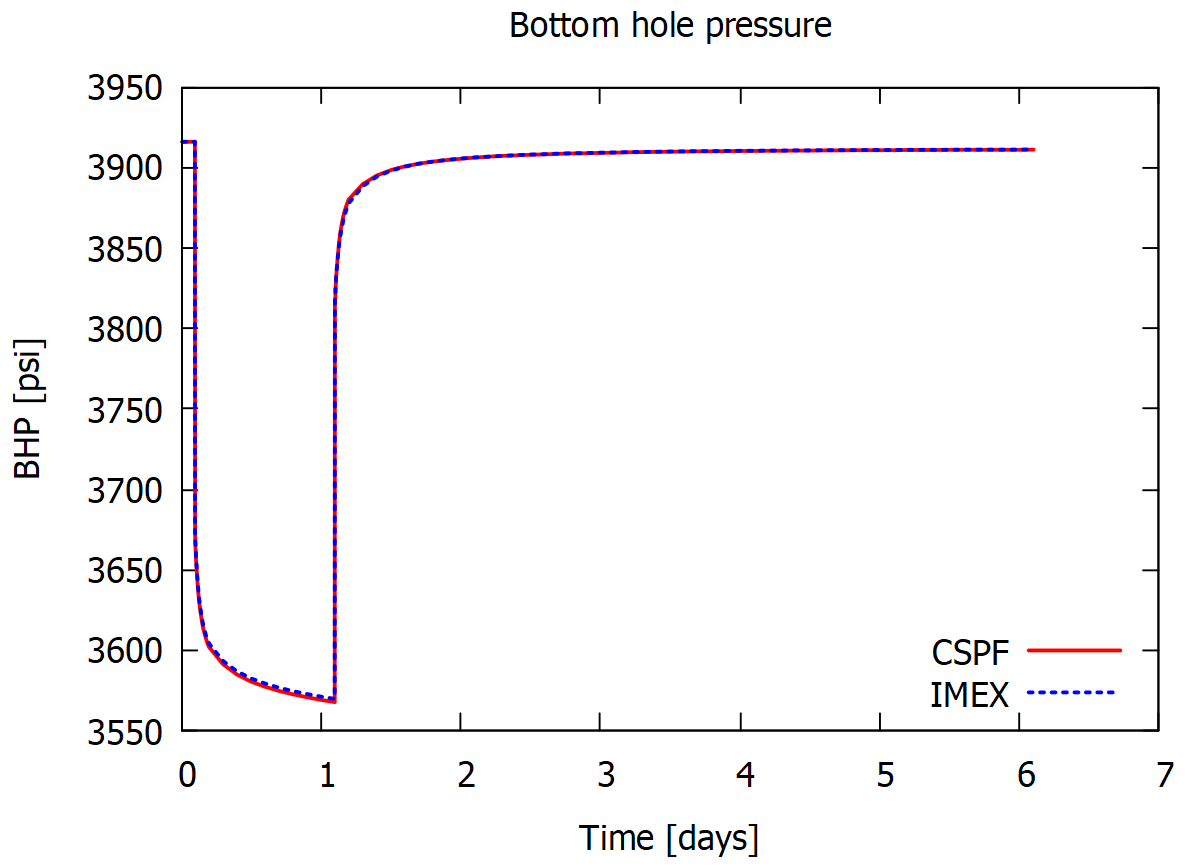
\includegraphics[width=0.8\linewidth]{24.png}
	\caption{Comparison between the CSPF and IMEX for a drawdown/buildup well test in a homogeneous reservoir.}
	\label{fig:24}
\end{figure}

Between 0 and 0.1 day, the well is closed, therefore its bottom hole pressure does not change. When the production starts, the BHP gets a steep decline until the production ceases. Then, the pressure raises again, stabilizing itself with asymptotic behavior. The difference between the initial stable BHP and the value stabilized after the test is proportional to the amount of oil produced in the reservoir, due to the fact that the production of oil will cause a depletion in the reservoir. One could see that the results from CSPF and IMEX are very close. A similar simulation has been done for the heterogeneous scenario, its results are shown in Figure \ref{fig:25}.

\begin{figure}[h]
	\centering
	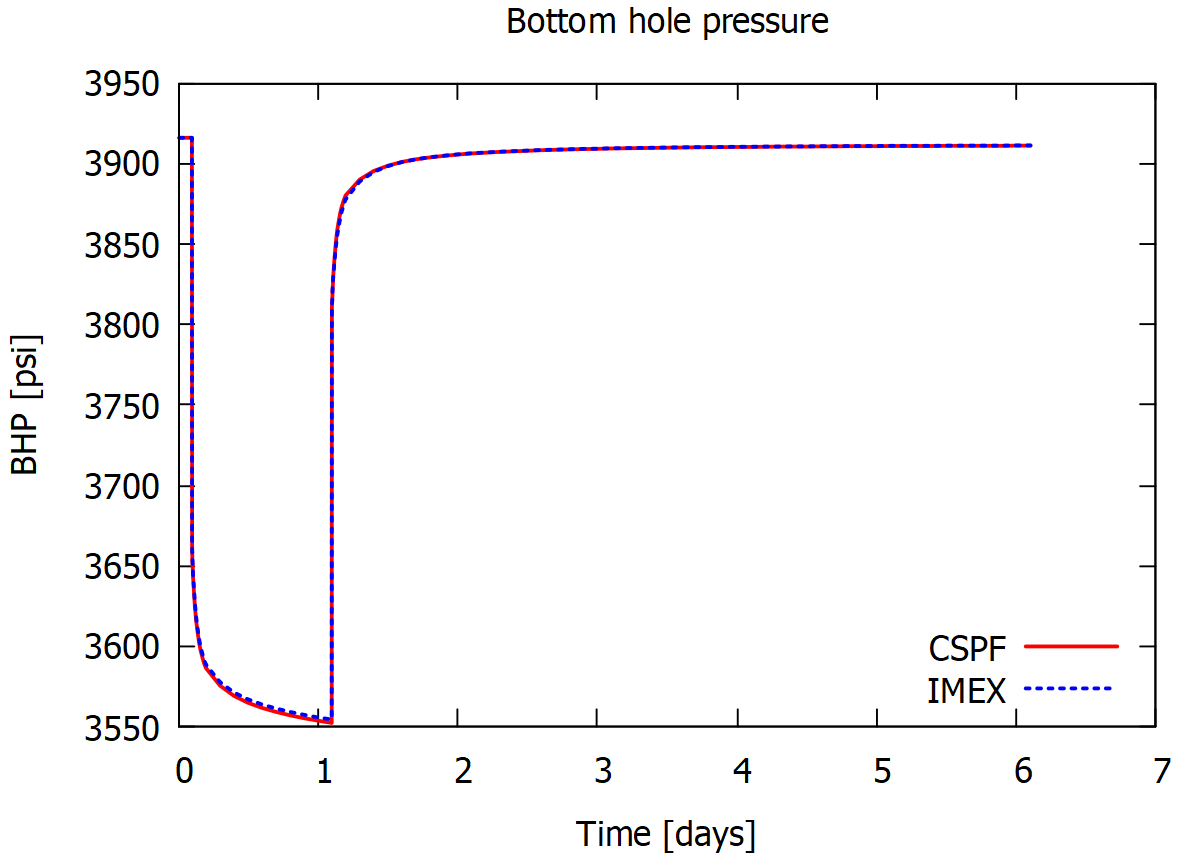
\includegraphics[width=0.8\linewidth]{25.png}
	\caption{Comparison between the CSPF and IMEX for a drawdown/buildup well test in a heterogeneous and anisotropic reservoir.}
	\label{fig:25}
\end{figure}

Looking at the results for the heterogeneous case in Figure \ref{fig:25}, one could see a modest change in comparison to the homogeneous results shown by Figure \ref{fig:24}. One difference is the minimum BHP, which is slightly lower in the second case. Again, the CSPF results are very similar to IMEX´s.

The difference between IMEX and CSPF for both scenarios has been plotted and displayed in Figure \ref{fig:29}. One explanation for these disparities could be the rounding dissimilarities between IMEX and CSPF, but overall the results are very similar. When juxtaposing the Figure \ref{fig:29} with the Figures \ref{fig:24} and \ref{fig:25}, one could note that the relative differences are higher when the BHP variation is steeper.
\begin{figure}[h]
	\centering
	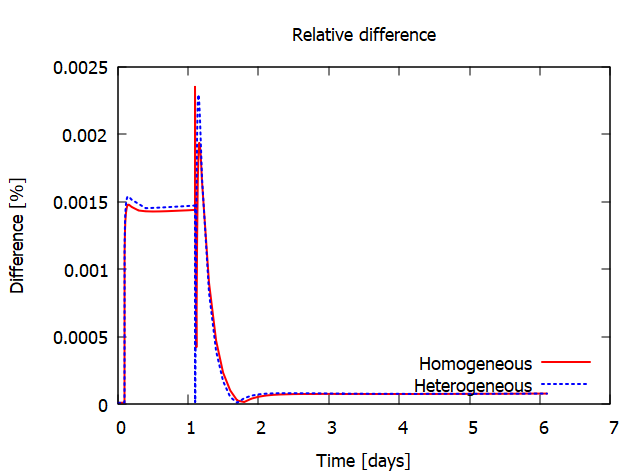
\includegraphics[width=0.8\linewidth]{29.png}
	\caption{Relative differences between CSPF and IMEX for the heterogeneous and homogeneous cases.}
	\label{fig:29}
\end{figure}


